% !TEX root = main.tex

\section{Lecture 7: Numerics: Time-stepping schemes}
\begin{flushright}\textbf{[by Xihan Zhang]}\end{flushright}

{\color{red}[Navid: Xihan, I made some small editorial comments and added 1-2 explanatory sentences. Have a look and tell me if all is OK.]}

In this lecture, we consider how models time-step forward in time by using finite difference method. 


Take the evolution of thickness $h(\boldsymbol{x}, t)$ in a layered model that was derived in lecture~\ref{sec:lecture5}: 

\begin{equation}
\frac{\partial h}{\partial t}+\frac{\partial (uh)}{\partial x}+\frac{\partial (vh)}{\partial y}=0 .
\label{layereqn}
\end{equation}

Since we want to know how thickness $h$ evolves with time, we rearrange \eqref{layereqn} as 

\begin{equation}
\frac{\partial h}{\partial t}=\underbrace{-\frac{\partial(uh)}{\partial x}-\frac{\partial (vh)}{\partial y}}_{\equiv F(\boldsymbol{x}, t)}.
\label{tmstep}
\end{equation}

We collectively denote all term on the right-hand-side above as $F$.

Now, let's consider a discretization of time into equal increments:
\begin{equation}
	0, \Delta t, 2 \Delta t, \dots, \tau \Delta t, \dots, \label{eq7.3}
\end{equation}
where $\tau$ is an integer. This way the $\tau$-th discrete time corresponds to value $t=\tau\,\Delta t$, $\tau=0,1,\dots$. We denote, hereafter, all field values at $t=\tau\,\Delta t$ simply with a subscript $\tau$, e.g.,
\begin{equation}
	h(\boldsymbol{x}, \tau\,\Delta t) \leftrightarrow h_\tau(\boldsymbol{x}),
\end{equation}
and similarly for $u$, $v$, $F$, etc. Thus, \eqref{tmstep} becomes
\begin{equation}
	\frac{\partial h_\tau}{\partial t} = F_\tau. \label{Ftau}
\end{equation}

What we need to do is to find a way to approximate the time-derivative $\partial h_\tau/\partial t$ on the left-hand-side above within our discrete time-domain~\eqref{eq7.3}.


\subsubsection*{Forward difference time-stepping scheme}

By definition, the continuous version of the time-derivative is:
\begin{equation}
\frac{\partial h_{\tau}}{\partial t}=\displaystyle \lim_{\delta t\to 0}\frac{h(\tau\,\Delta t+\delta t)-h(\tau\,\Delta t)}{\delta t}.
\label{dhdt}
\end{equation}

The discretised approximation of \eqref{dhdt}, after we take $\delta t = \Delta t$, becomes:
\begin{equation}
\frac{\partial h_{\tau}}{\partial t} \approx \frac{h_{\tau +1}-h_{\tau}}{\Delta t}.
\label{dhdt1}
\end{equation}

To obtain the forward step for $h$, combine \eqref{Ftau} and \eqref{dhdt1}, 
\begin{equation}
h_{\tau+1}=h_{\tau}+\Delta t F_{\tau}.
\label{fdt}
\end{equation}
The time-step above is called `forward difference'. The schematic diagram of this calculation is shown in Fig.~\ref{fddiagram}.
\begin{figure}[h!]
\centering
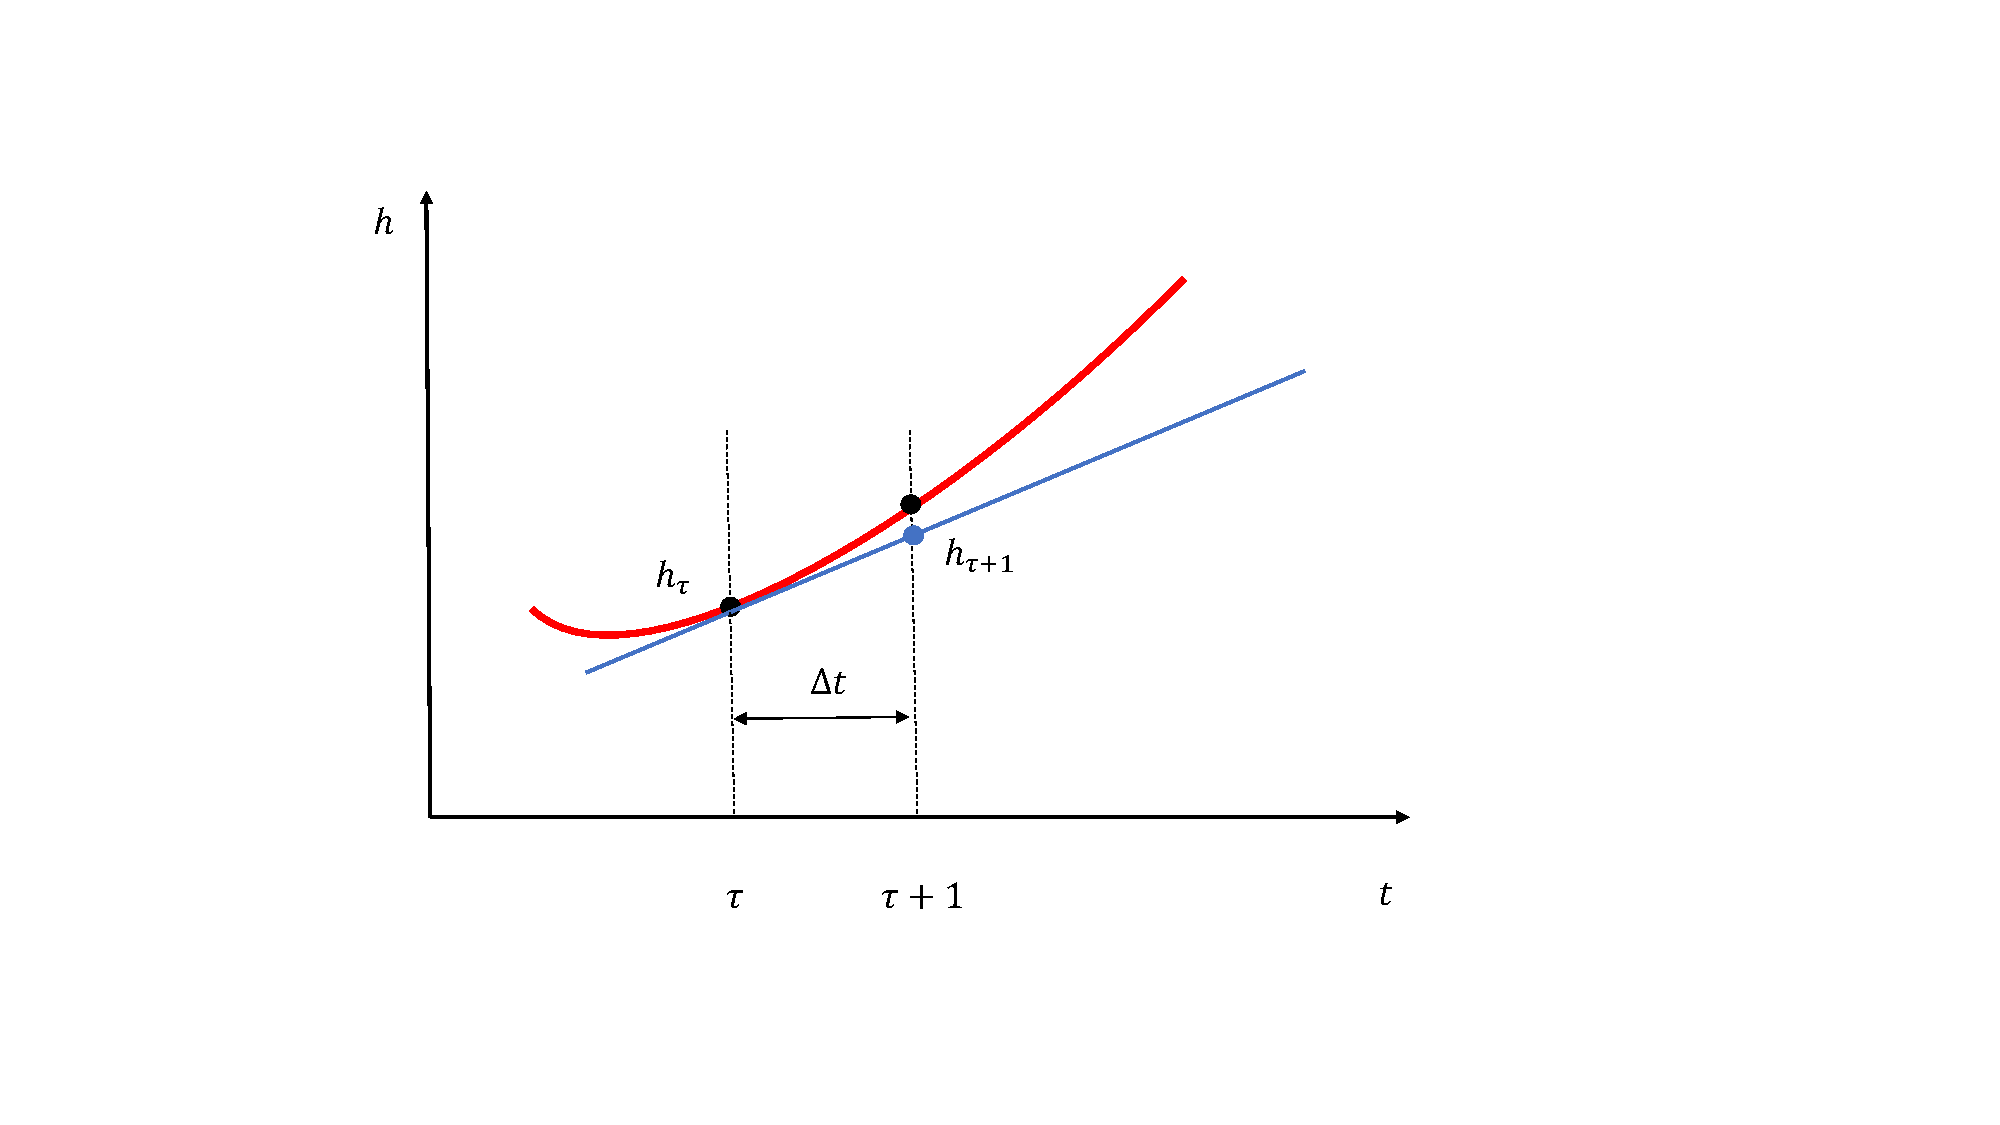
\includegraphics[width=0.6\textwidth]{lecture7-fig1}
\caption{Forward difference method}
\label{fddiagram}
\end{figure}

Note that above the only approximation was done in~\eqref{dhdt1}. We would like to have a way to estimate the error that we made using~\eqref{dhdt1}. Intuitively, one should expect that the error should decrease as we take smaller $\Delta t$, but how fast does the error approaches zero?

To can quantify the performance of a time-stepping scheme, using Taylor series. Recall that any infinitely differentiable function $f(x)$ can be expanded  in a Taylor series as: 
\begin{equation}
f(x_0+a)=f(x_0) + \left.\frac{\partial f}{\partial x}\right|_{x=x_0} a + \left.\frac{\partial^{2}f}{\partial x^{2}}\right|_{x=x_0}\frac{a^{2}}{2!} + O(a^{3}).
\label{TS}
\end{equation}

Applying this to $h$ by taking $x_0=\tau\,\Delta t$ and $a=\Delta t$, we have that
\begin{equation}
h_{\tau+1}=h_{\tau}+\frac{\partial h_{\tau}}{\partial t}\Delta t + O(\Delta t^{2}).
\label{htTS}
\end{equation}

After rearranging terms in \eqref{htTS} and dividing by $\Delta t$,
\begin{equation}
\underbrace{\frac{h_{\tau+1}-h_{\tau}}{\Delta t}}_{(i)}=\underbrace{\frac{\partial h_{\tau}}{\partial t}}_{(ii)} + \underbrace{O(\Delta t)}_{(iii)}.
\label{FOA}
\end{equation}


Since term $(ii)$ the time-derivative of $h$ at $\tau\Delta t$ and term $(i)$ is approximation~\eqref{dhdt1} of this time-derivative, the discrepancy between them expressed in term $(iii)$ is the error. The error for `forward difference' is proportional to $\Delta t$: we say that `forward difference' is a `first-order time-stepping scheme' or is `first order accurate', which means the error decreases linearly with the decrease of the time step. 

Can we do any better? Can we use a different approximation of the time-derivative instead of~\eqref{dhdt1} so that the error is much less?

\subsubsection*{Leapfrog time-stepping}


Instead of using $h_{\tau}$ and $h_{\tau+1}$ to estimate  the derivative, now we use $h_{\tau-1}$ and $h_{\tau+1}$ to do this, leading to 
\begin{equation}
\frac{\partial h_{\tau}}{\partial t}\approx\frac{h_{\tau+1}-h_{\tau-1}}{2\Delta t}.\label{eq7.12}
\end{equation}

This is known as `centred difference' or `leapfrog' method and the schematic diagram is shown in Fig.~\ref{CDdiagram}.
\begin{figure}[h!]
\centering
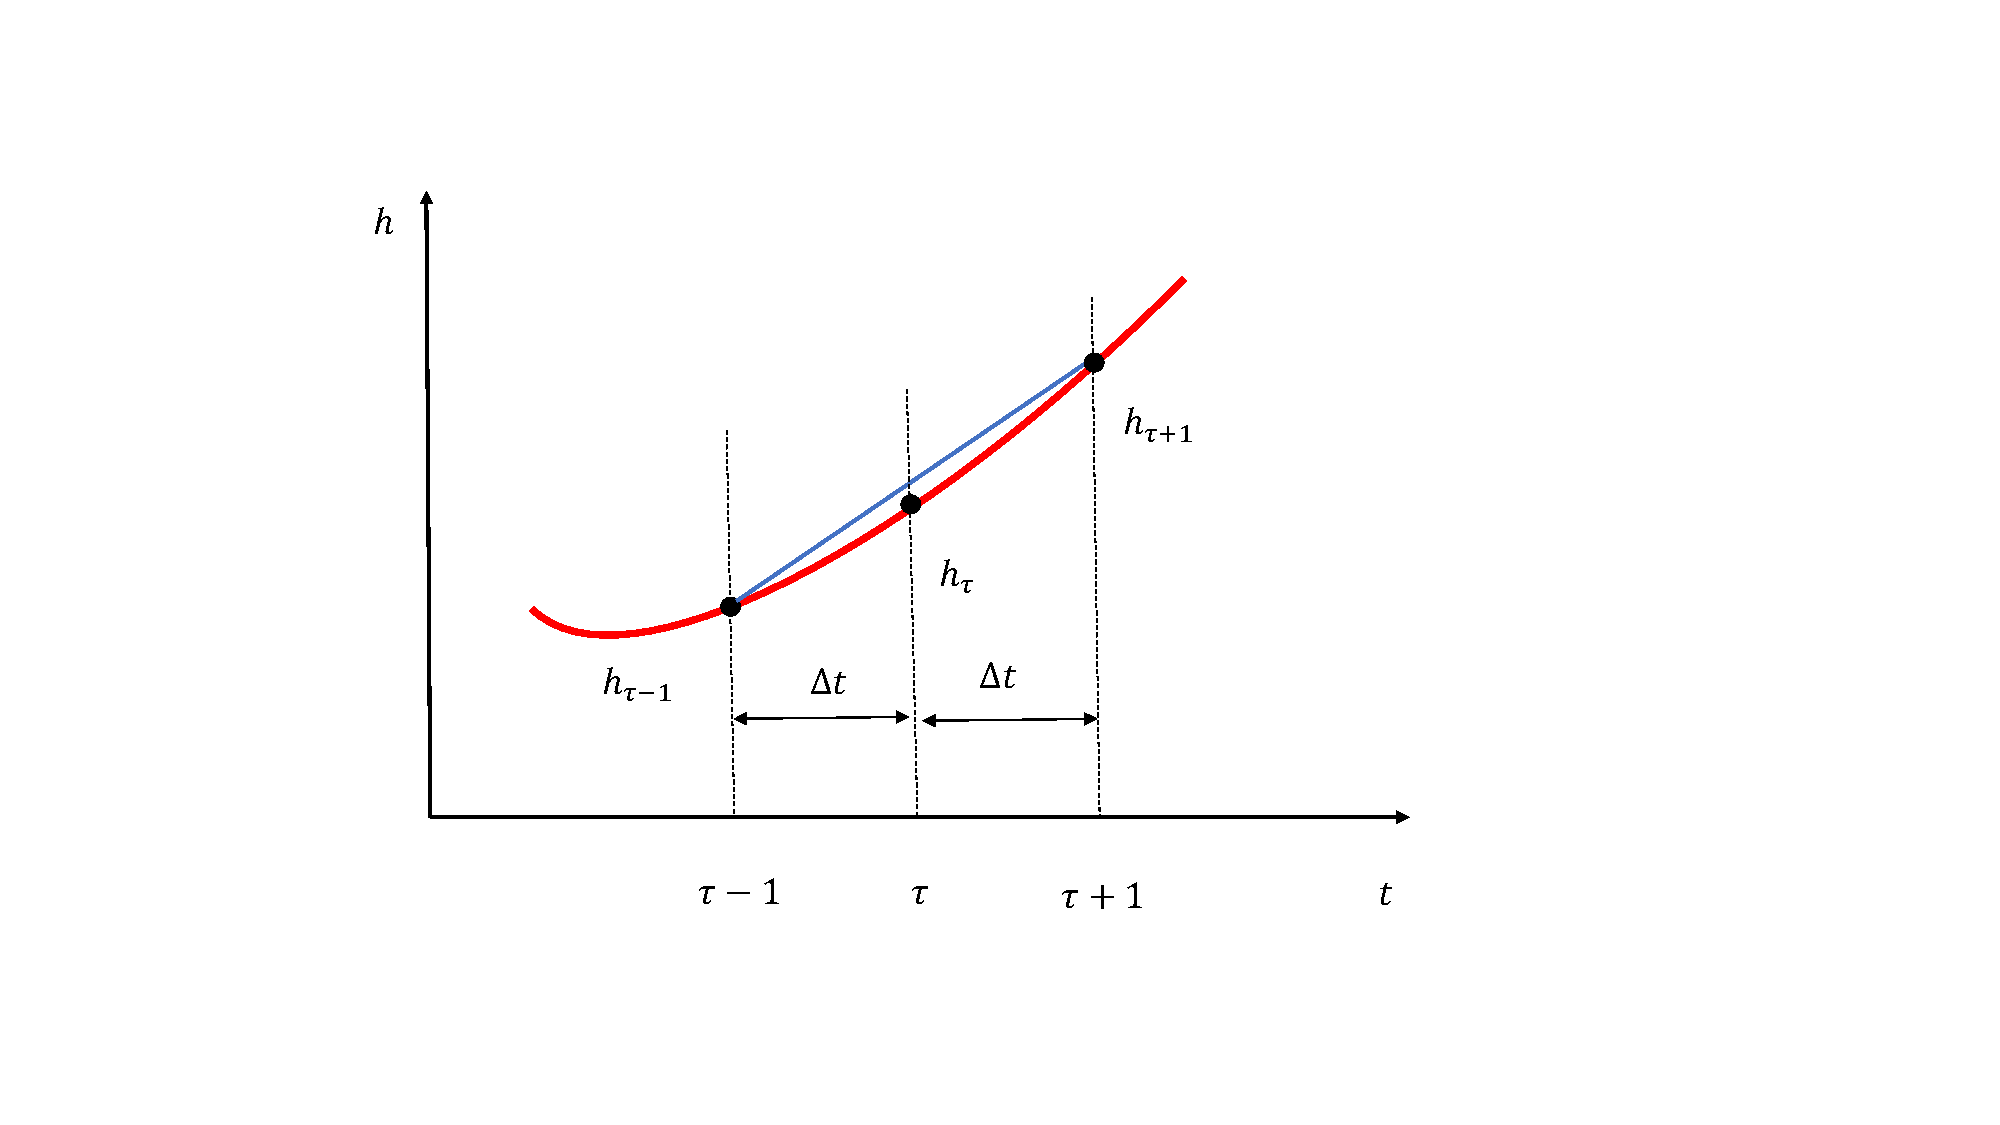
\includegraphics[width=0.5\textwidth]{lecture7-fig2}
\caption{Centred difference method.}
\label{CDdiagram}
\end{figure}

Now, we can repeat the same steps as before to estimate the error we make using~\eqref{eq7.12}. Expand $h_{\tau+1}$ and $h_{\tau-1}$ as a Taylor series:

\begin{align}
	h_{\tau+1}&=h_{\tau}+\frac{\partial h_{\tau}}{\partial t}\Delta t+\frac{\partial^{2}h_{\tau}}{\partial t^{2}}\frac{\Delta t^{2}}{2}+O(\Delta t^{3}),\\
	h_{\tau-1}&=h_{\tau}-\frac{\partial h_{\tau}}{\partial t}\Delta t +\frac{\partial^{2} h_{\tau}}{\partial t^{2}}\frac{\Delta t^2}{2}+O(\Delta t^{3}),
\end{align}

and then subtract them and divide by $2\Delta t$ to form the time-derivative approximation in~\eqref{eq7.12}. We obtain: 
\begin{equation}
	\underbrace{\frac{h_{\tau+1}-h_{\tau-1}}{2\Delta t}}_{(i)}=\underbrace{\frac{\partial h_{\tau}}{\partial t}}_{(ii)}+\underbrace{O(\Delta t^{2})}_{(iii)}.
\label{SOA}
\end{equation}

Similarly as with the forward difference, term $(iii)$ is the error of centred difference method. This time the error is proportional to $(\Delta t)^2$, which is much smaller than $\Delta t$ for small time-steps. Therefore, `centred difference' is second-order accurate and the error declines quadratically as we decrease of the time-step. 

\subsubsection*{A small catch}

The advantage of this `leapfrog' method of time stepping is that it is second order accurate, but it can also induce instability as there are two independent  subsets of the discretised $h_{\tau}$ values that evolve independently without interaction, sometimes leading, possibly, to divergence at some point. Figure~\ref{leapfrog} depicts disconnect between subsets values at $\tau, \tau+2,\tau+4, \dots$ and those at $\tau+1, \tau+3, \dots$: the time grid splits into two subsets (here shown with black and blue) of two independent solutions resulting to numerical instability.

\begin{figure}[h!]
\centering
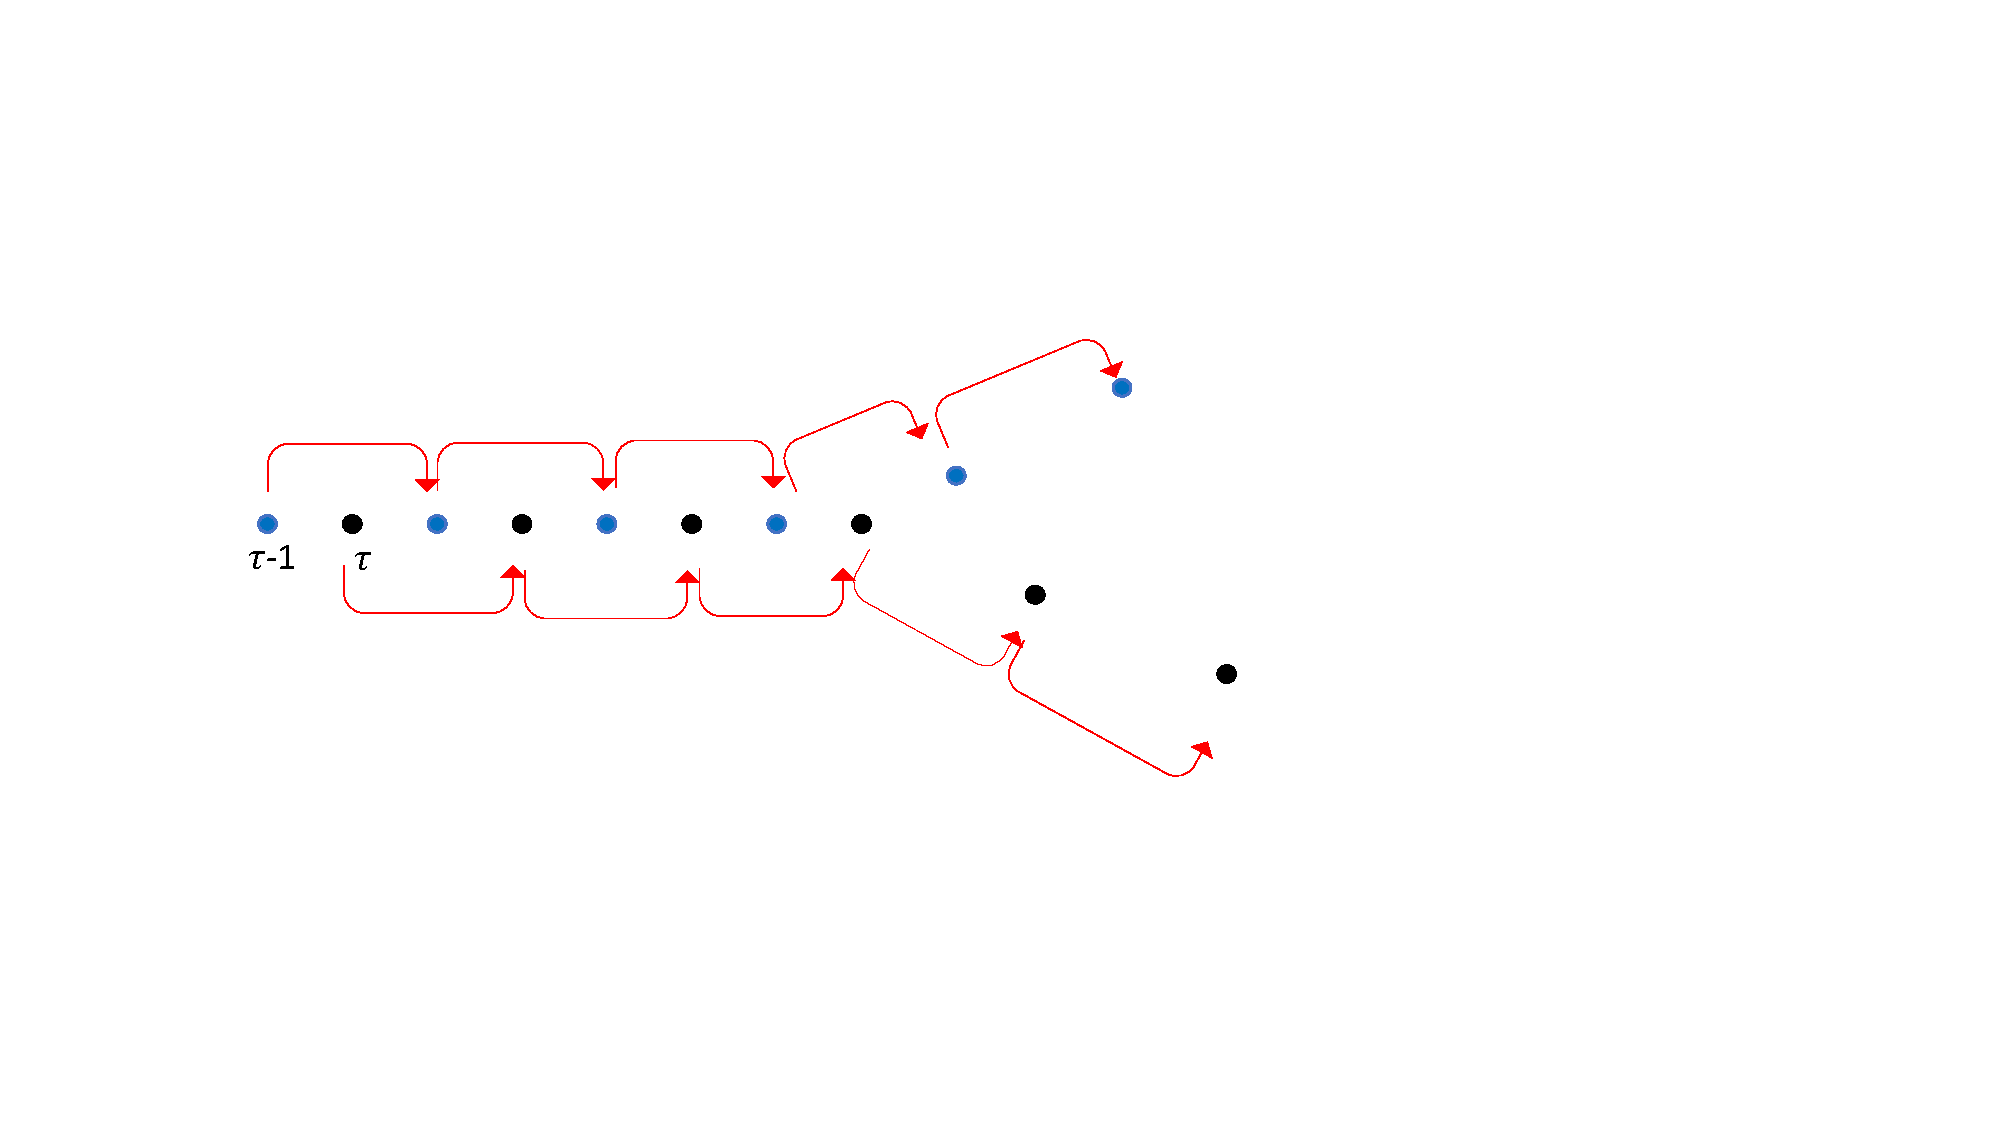
\includegraphics[width=0.5\textwidth]{lecture7-fig3}
\caption{Schematic of numerical instability due to the miscommunication of two different subsets of time-grids when using the leapfrog time stepping scheme.}
\label{leapfrog}
\end{figure}

Therefore, it is necessary to `mix' these two solutions at neighbouring time grid-points to resolve this issue of numerical divergence. To do so, we usually implement a filter on each leapfrog time step. The filter that is  most commonly used is the Robert--Asselin filter:
\begin{equation}
h_{\tau-1}^{R}=h_{\tau-1}+\alpha(h_{\tau}-2h_{\tau-1}+h_{\tau-2}^{R}),
\end{equation}
where $h^{R}$ represents filtered variables. 

We note that implementing Robert-Asselin filter \emph{does} resolve the issue with numerical instability due to the disconnect of the two different time-grid subsets but does come at the expense of the accuracy (the error becomes more than $O(\Delta t)^2$). 
